% !TEX root = ../aas_submission.tex
\documentclass[../main.tex]{subfiles}
\begin{document}
\label{sec:results}

In this Section we explore the consistency with which volunteers modelled galaxies, the accuracy of the aggregate models, and compare the aggregate and fitted models to comparable results in the literature.

\subsection{The Calibration Set}

The recovered models for the nine synthetic galaxy images created for the \textit{calibration subset} show that volunteers make systematic use of bulges, even when only a bar component is needed, resulting in two Type 1 errors for bulge presence in the aggregate model. It also highlighted the limitation of the Jaccard metric for highly elliptical components (bars), as even a small change in rotation results in a large change in the metric. The result of this is one Type 2 error of bar presence in the aggregate. We successfully recover all spiral arms present, and do not receive any false positives. The pitch angles obtained through aggregation vary by up to $9^\degree$ from the true values, with fitting improving the error slightly.

Fitting also highlighted the difficulty in recovering structural parameters for which we did not obtain a starting point through clustering (S\'ersic index and bar boxyness). These parameters are crucial for measurements of bulge fraction, but difficult to identidy using gradient descent \comment{citation needed}. Reduced Chi-squard values for the fits range from 1.00 to 1.33 (where degrees of freedom has been estimated as the number of unmaked pixels in the image, as in \citealt{galfit-paper}).

As these galaxies were used to fine-tune clustering and fitting hyperparameters, our ability to recover morphology accurately is essential validation for our ability to recover good photometic models of galaxies. These results highlight the importance of good priors to obtain accurate fits of complex photometric models.


\subsection{Examination of Volunteer consistency}
We aggregate two independent models for a set of 98 galaxies based on ``original'' or repeat (``validation'') classifications, obtained with the same retirement limit (see Section \ref{sec:retirement-limit} for more on this selection).

One of the simplest choices the volunteers have is whether to include a model component or not. Figure \ref{fig:volunteer_component_consistency} illustrates the consistency with which volunteers made use of a component in their model for a galaxy. We see that volunteer classification is very consistent, with scatter as predicted by the Binomial uncertainty on the mean. Volunteers almost always make us of a disc and bulge (as seen in the \textit{calibration subset}), and even proportions agree on the presence of a bar and the number of spiral arms. Many volunteers used a very elliptical bulge and the ends of spiral arms to model light that could be seen classified as a bar. The validation model is identical to the original model for less 40\% of galaxies (often due to a missing bar component or single spiral arm), suggesting further work is needed to ensure consistency in aggregation.

\begin{figure*}
  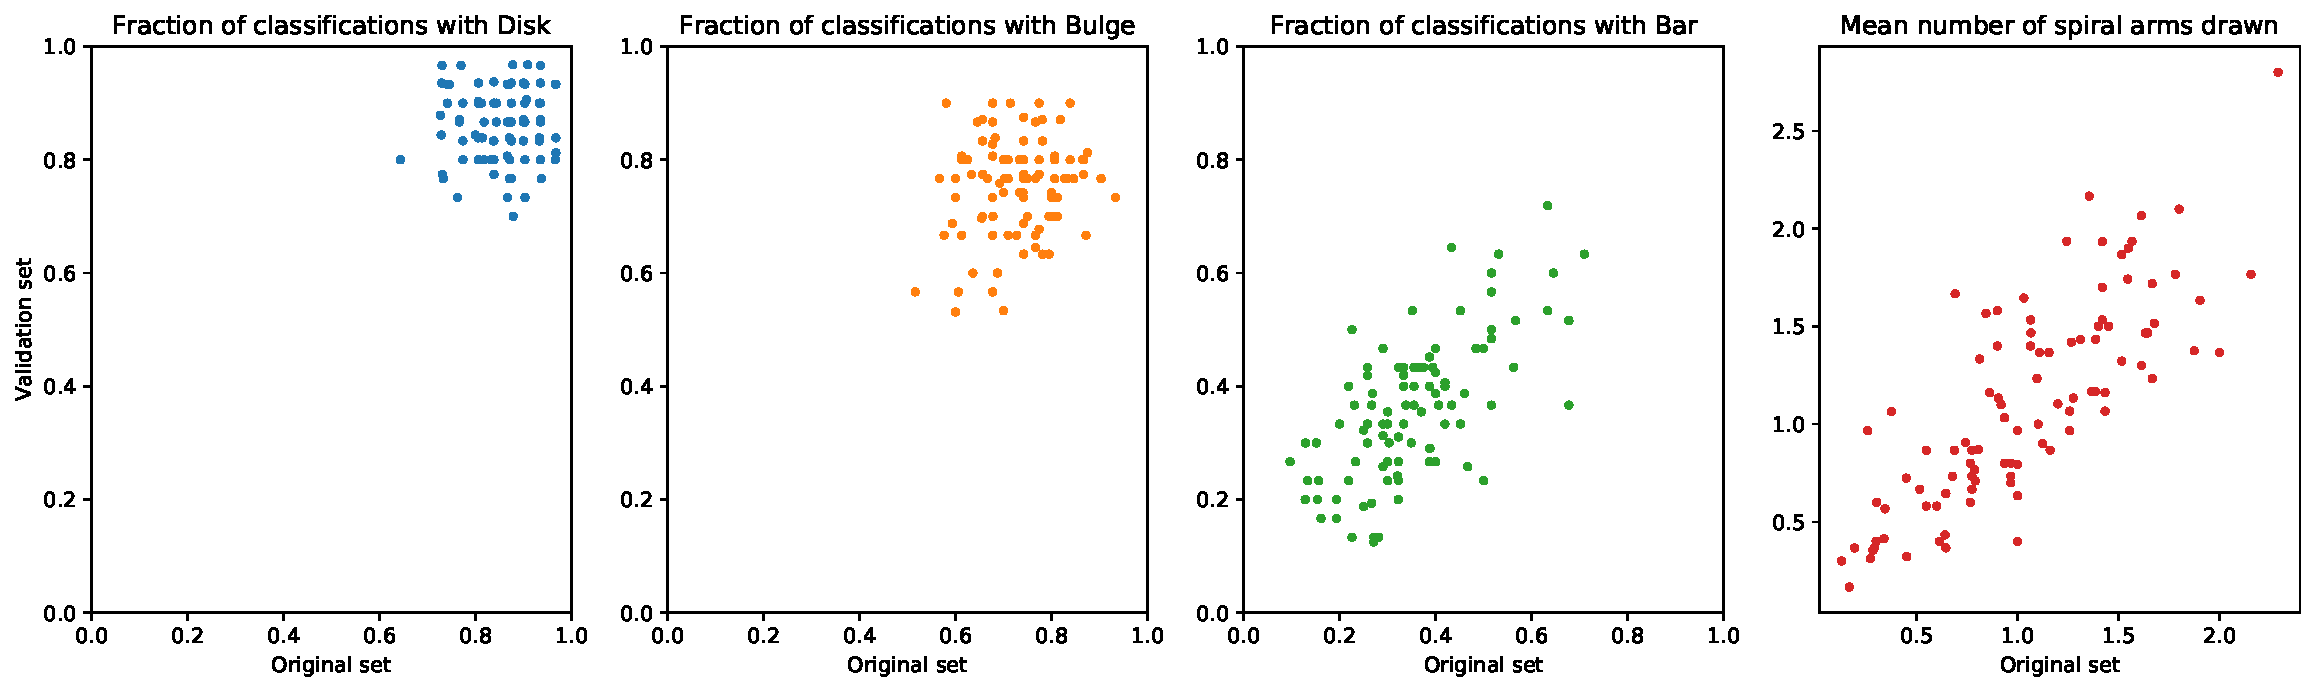
\includegraphics[width=17.3cm]{images__results/component_frequency.pdf}
  \caption{Comparison of frequency of use of component in volunteer models between the original and validation sets of classifications. Errors shown on the disc, bulge and bar arise from Binomial error estimation.}
  \label{fig:volunteer_component_consistency}
\end{figure*}

After selecting a component, the volunteer sets its shape and size. Fewer bars being drawn by volunteers makes clustering more difficult and more uncertain; for a strongly barred galaxy with 30 classifications we recieve only 15 or so drawn bars. The variation in axial ratios and effective radii for the aggregate discs, bulges and bars are shown in Figure \ref{fig:aggregate_model_consistency}. The aggregate disks and bulges are consistent within errors, while bars show more scatter, potentially due to reasons discussed above.

\begin{figure*}
  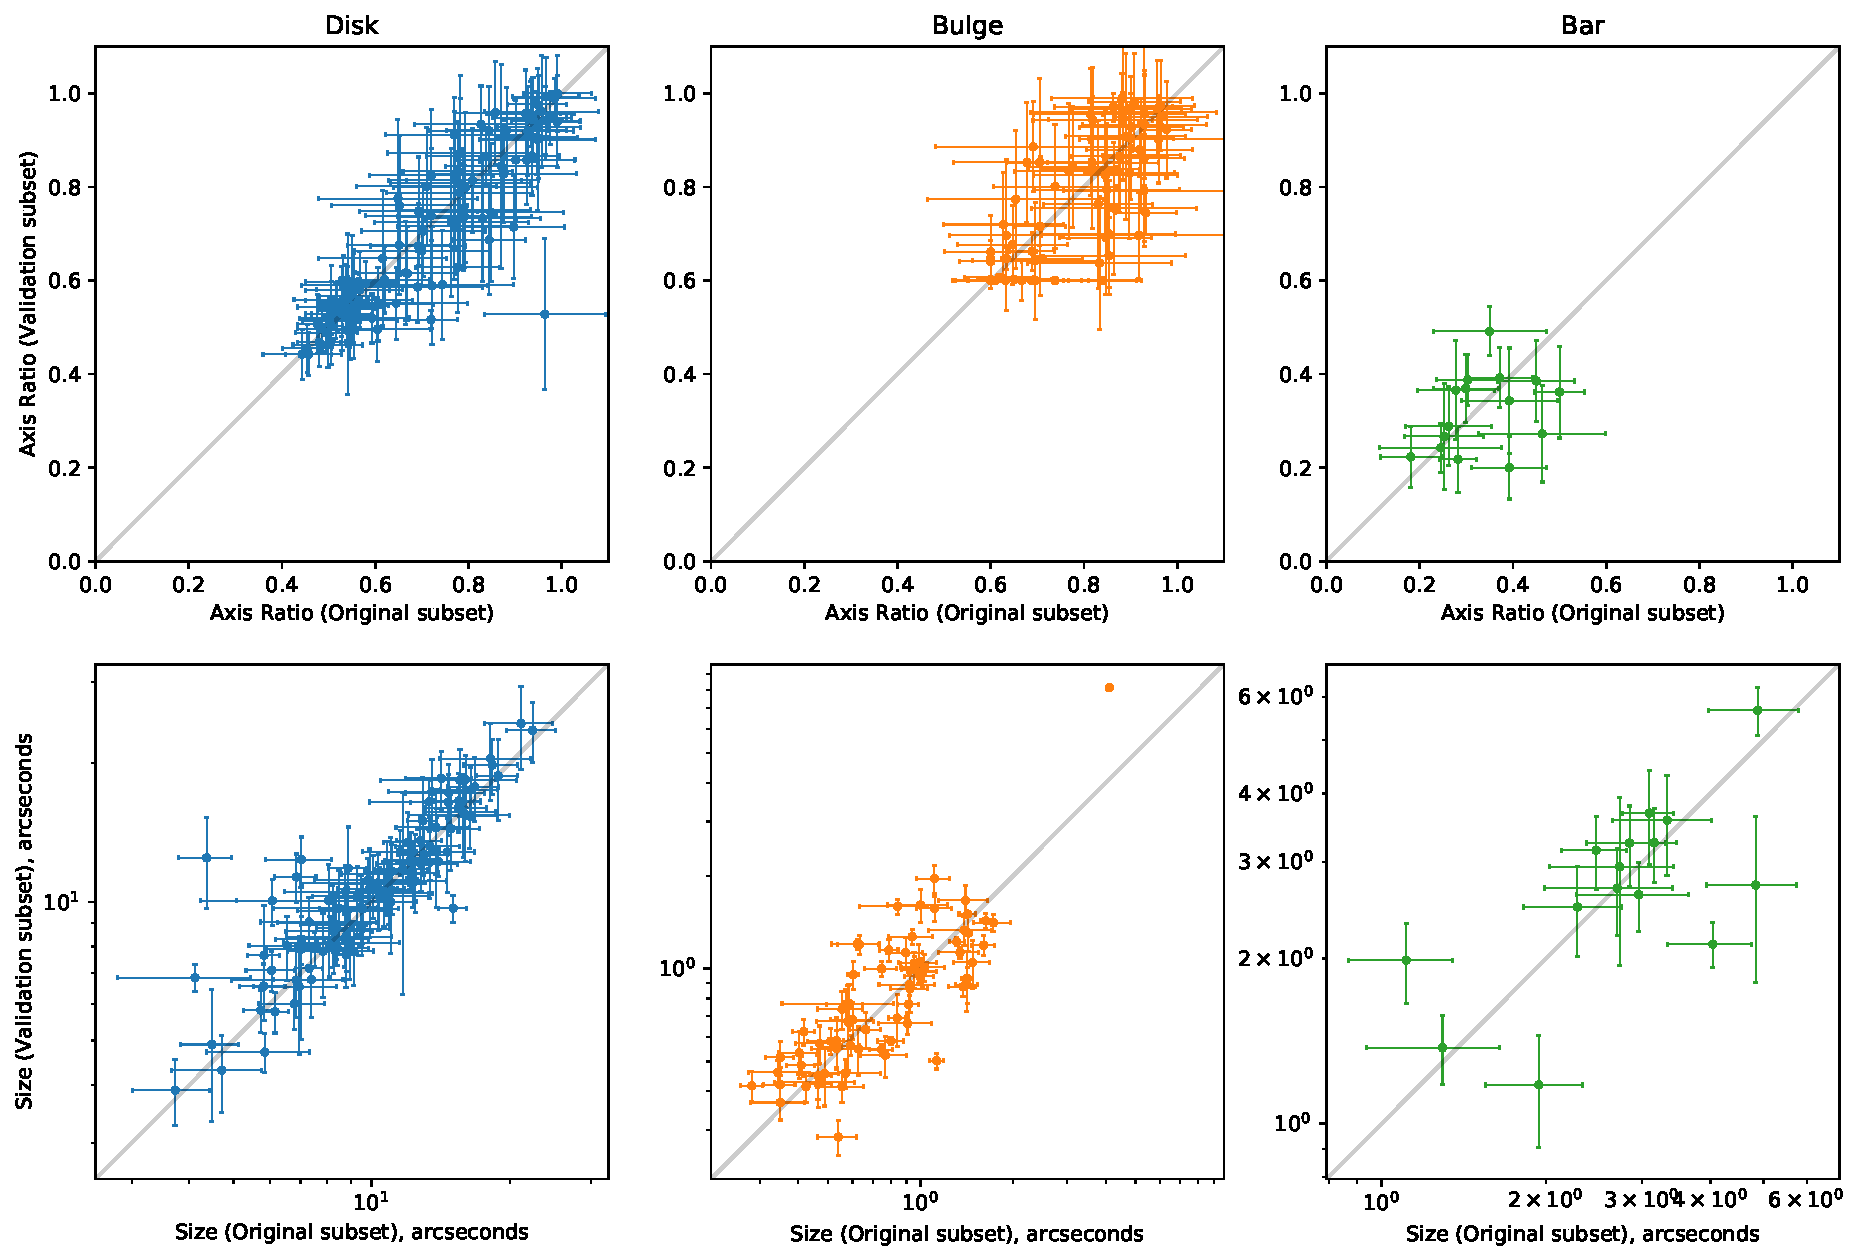
\includegraphics[width=17.3cm]{images__results/component_sizing.pdf}
  \caption{Comparison of component shape in aggregate models between the original and validation sets. Errors are obtained through the sample variance of clustered components, as detailed in Section \ref{sec:error_estimation}.}
  \label{fig:aggregate_model_consistency}
\end{figure*}

\subsection{Comparison to results in the literature}

After having obtained aggregated models for our galaxies, we examine how our models compare to other results in the literature. There exists no published comparison sample with four-component fits, instead we make comparisons for individual or subsets of model components.

\subsubsection{Comparison to Galaxy Zoo morpohology}

The simplest comparison we can make to external results is to examine whether our models respect the existing morpohological classifications present in the literature. We make use of Galaxy Zoo 2 (GZ2, \citealt{Willett2013:1308.3496v2}) results, including the redshift debiasing described in \citet{Hart2016:1607.01019v1} and spiral properties calculated in \citet{Hart2016:1607.01019v1}.

When comparing the probability of a volunteer's classification containing a bar component against a galaxy being classed as strongly-barred or as having no bar (as defined in \citealt{Masters2010:1003.0449v2}), we see a significant difference: ignoring Binomial uncertainty, classifications of strongly-barred galaxies ($p_\text{bar} > 0.5$) had a $0.47 \pm 0.15$ chance of containing a bar, vs $0.29 \pm 0.11$ for galaxies classed as having no bar ($p_\text{bar} < 0.2$). The Pearson correlation between GZ2's $p_\text{bar}$ and the bar likelihood in \textit{Galaxy Builder} is $0.56$, implying a significant correlation. We do not compare to the morphology of the aggregate model as we tuned the bar clustering hyperparameters using GZ2 morphologies.

We also compare the number of spiral arms aggregated by \textit{Galaxy Builder} with the responses to the GZ2 ``number of arms'' question (of which the possible responses were one, two, three, four, more than four or ``Can't tell''). We attempt to account for the spread in volunteer answers to this question by binning responses, rather than using the mean or modal response. The results of this comparison can be seen in Figure \ref{fig:n_spirals_comparison}. The area of each circle can be seen as the level of agreement between \textit{Galaxy Builder} aggregate models and GZ2 classifiers, it is defined as

\begin{equation}
  \label{eq:spiral_circle_area_size}
  A_{i, j} \propto \sum_{k}^{N_g}\frac{1}{M_k}\sum_{m}^{M_k}
  \begin{cases}
    1,&\ \mathrm{if}\ n_k = i\ \mathrm{and}\ C_{k, m} = j\\
    0,&\ \mathrm{otherwise}
  \end{cases},
\end{equation}

where $n_k$ is the number of aggrage arms for galaxy $k$ (out of $N_g$ galaxies), $C_{k, m}$ is the $m$-th answer for galaxy $k$ (out of $M_k$ answers).

The circle with the largest area for each possible GZ2 response is highlighted, and agrees with the number of spiral arms aggregated here for $m=1, 2, 3, 4$. No aggregate model contained more than four spiral arms, and when galaxies have an uncertain number of spiral arms (the ``Can't tell'' GZ2 response) we mostly do not aggregate any spiral arms.

It is not uncommon in \textit{Galaxy Builder} for one spiral arm to have been broken into two smaller segments. We also occasionally identify two distinct clusters that represent the same physical arm. These two reasons account for a majority of cases where GZ2 classifications suggest a galaxy has two spiral arms and we have identified a larger number.

\begin{figure}
  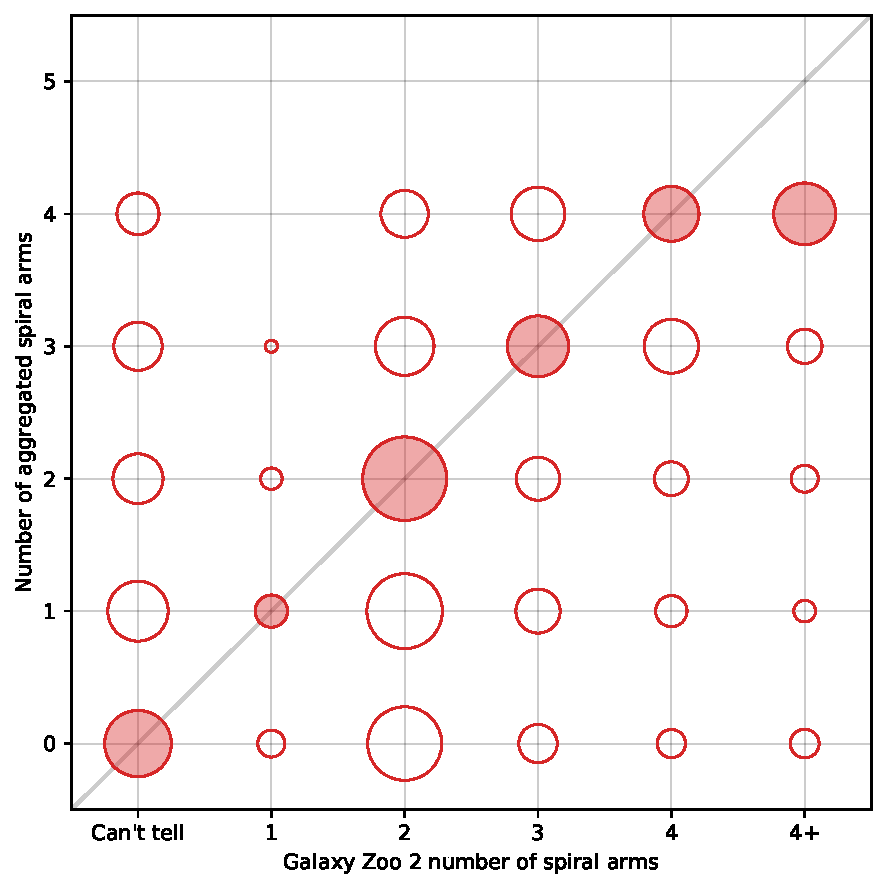
\includegraphics[width=8cm]{images__results/spiral-number-vs-gz2.pdf}
  \caption{Density plot of GZ2 vote counts for spiral arm number vs the number of spiral arms obtained through aggregation. The area of each circle can be seen as the level of agreement between \textit{Galaxy Builder} aggregate models and GZ2 classifiers, and is defined by Equation \ref{eq:spiral_circle_area_size}. The circle with the largest area for each possible GZ2 response is highlighted by shading.}
  \label{fig:n_spirals_comparison}
\end{figure}


\subsubsection{Comparison to One-component fit - axis ratio}
We compare the axis ratios of the discs of \textit{Galaxy Builder} aggregate models (without tuning) to the axis ratio of a 2D S\'ersic fit to the r-band SDSS image of each galaxy (as provided in the NSA catalog, \citealt{2011AJ....142...31B}). We see excellent (Figure \ref{fig:ax_ratio_comparison}).

For the untuned models there is an error of $\sim0.1$, consistent with our expected errors (derived in Section \ref{sec:error_estimation}). There is a clustering of outlying values at $b/a=0.5$ which is almost certainly due to the drawing tool ellipse having a default axis ratio of 0.5. Where this default is a ``good enough'' fit we hypothesise that volunteers are less likely to modify it, while if it needs to move a long way they find a more refined value.

Volunteers not adjusting components from their default values was a consistent issue with untuned models (36\% of all disc components drawn by volunteers were left at the default axis ratio, and over half of all bars were left with their default rotation, though many of these would have been excluded during clustering). Future projects should carefully consider their interface design to minimize this bias. Fitting aggregate models successfully removes this bias though the overall scatter does not change.

\begin{figure}
  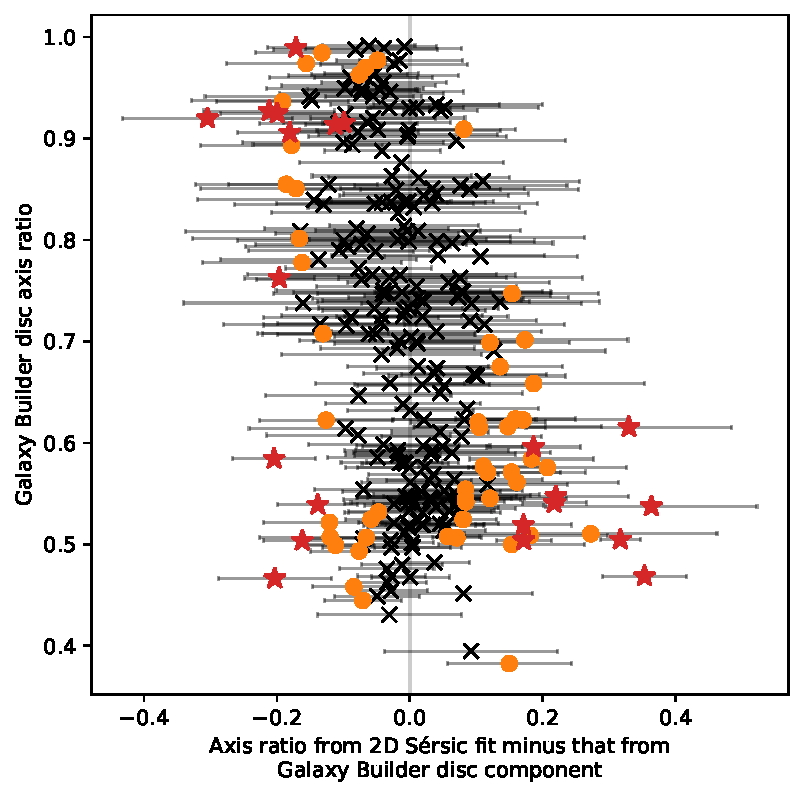
\includegraphics[width=8cm]{images__results/gzb-agg-nsa-comparison.pdf}
  \caption{Difference between the axis ratios of the aggregated disc component (before fitting) to the results of an r-band S\'ersic profile fit. Points  between one- and two-sigma are highlighted as orange squares, points outside two-sigma are shown as red stars.}
  \label{fig:ax_ratio_comparison}
\end{figure}


\subsubsection{Comparison to Disc-Bulge models}

A strong motivation for performing multi-component modelling is the desire to measure the fraction of a galaxy's light being emitted by its central components (such as bulge fraction, defined as the ratio of bulge luminosity to total luminosity). \citet{Gao2017:1709.00746v1} demonstrate that modelling secondary central components is essential for recovering an accurate measure of bulge fraction. The difficulty of measuring bulge fraction is further componded by the complex degeneracies present in even two-component fits, meaning that many gradient-descent based solvers often fail to find the globally optimum solution \comment{maybe cite \citep{profit-paper} or Simard}, especially when bulge S\'ersic index is a free parameter.

One of the largest catalogs of 2D multi-component fits is \citet{2011ApJS..196...11S}, which performed simultaneous, two-bandpass decompositions of 1,123,718 galaxies in the Legacy area of the SDSS DR7 using \textsc{Gim2D}. Three variations of models were fitted: a pure S\'ersic model, an Exponential disc and de-Vaucouleurs bulge model (hereafter exp+deV), and an Exponential disc and a S\'ersic bulge model (exp+S). Ftting was performed using the Metropolis algorithm, which is resilient to local minima and therefore suitable for the complex likelihood space of galaxy photometric modelling. \citet{2012MNRAS.421.2277L} similarly fitted two models to SDSS main-sample galaxies: an exponential disc and exponential bulge (exp+exp), and an exponential disc and de Vaucouleurs bulge. They used a Levenberg-Marquadt gradient descent algorithm, with initial parameters taken from previous SDSS analysis.

We compare our central component fraction to bulge fraction from \citet{2011ApJS..196...11S} where their analysis indicated genuine bulge+disc systems ($P_{pS} \le 0.32$). We compare to \citet{2012MNRAS.421.2277L} bulge fractions only when their criteria determined that model was the best-fit model. We see a significant scatter, but a strong correlation (Figure \ref{fig:bulge_fractions}). We note that the relationship to exp+deV models appears to be less than 1:1, while the relationship to exp+exp models is greater than 1:1, highlighting the dependance of bulge fraction on S\'ersic index. We also note that the amount of scatter (and lack of consistent 1:1 relationships) between the bulge fractions of two-component models is comparable to the scatter we see to our more complex one.

\comment{last sentence is a bit clunky}

\begin{figure*}
  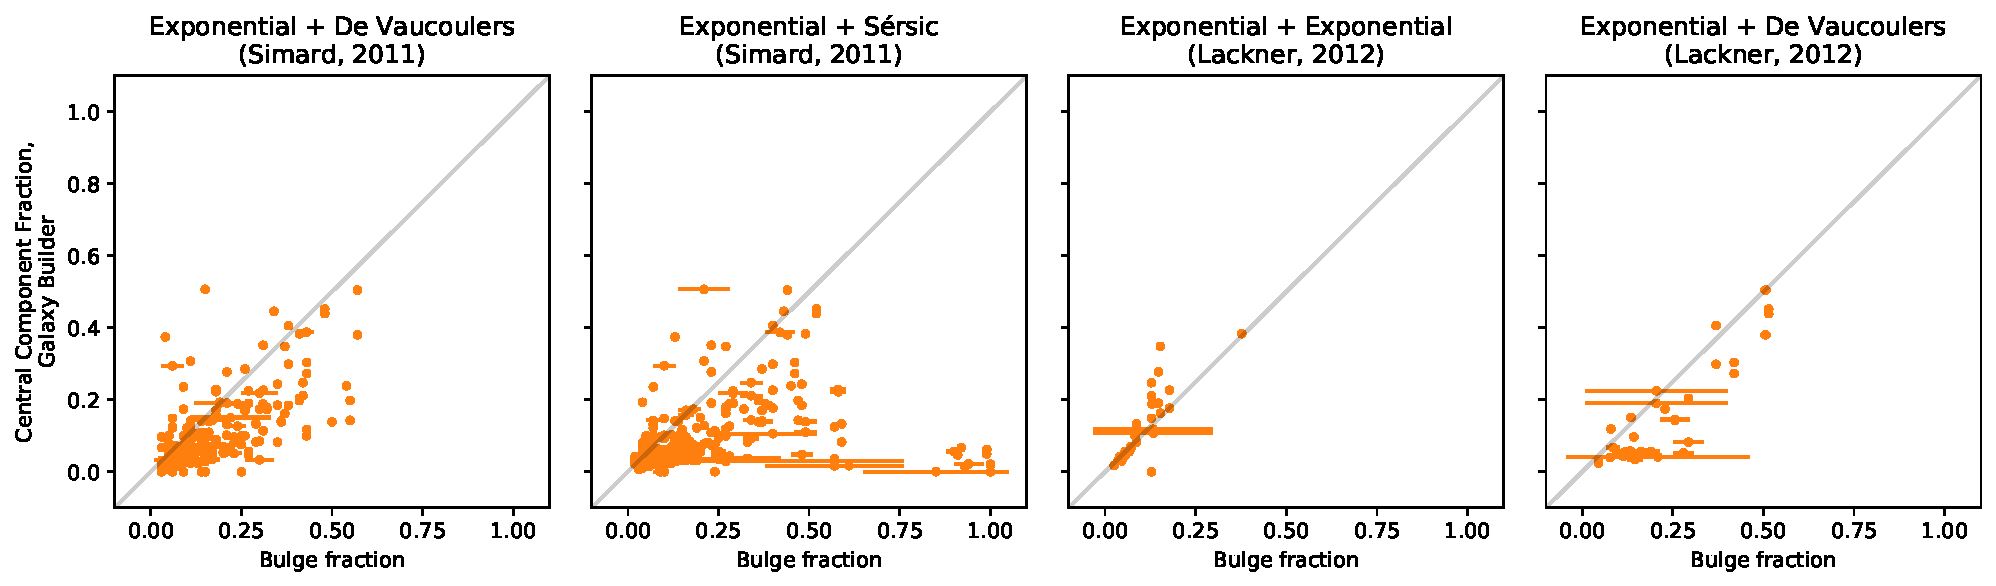
\includegraphics[width=17.3cm]{images__results/bulge_fraction_scatter_reduced.pdf}
  \caption{Scatter plots comparing the ratio of flux from central components (bulge and bar) to the total flux between fit models from \textit{Galaxy Builder} and two-component models in the literature.}
  \label{fig:bulge_fractions}
\end{figure*}


\subsubsection{Comparison to Disc-Bulge-Bar models}

\citet{2018MNRAS.473.4731K} performed multi-component, multi-band decompositions of a selection of SDSS galaxies, 12 of which were also classified in \textit{Galaxy Builder}. Figure \ref{fig:sd_comp_comparison} compares the axis ratios and effective radii of bulges, discs and bars in \citet{2018MNRAS.473.4731K} to those present in the aggregate models. We see strong consistency in all effective radii, with more scatter in component axis ratio. Comparing values for central component fraction as above, we see a near-identical 1:1 relationship.

\begin{figure}
  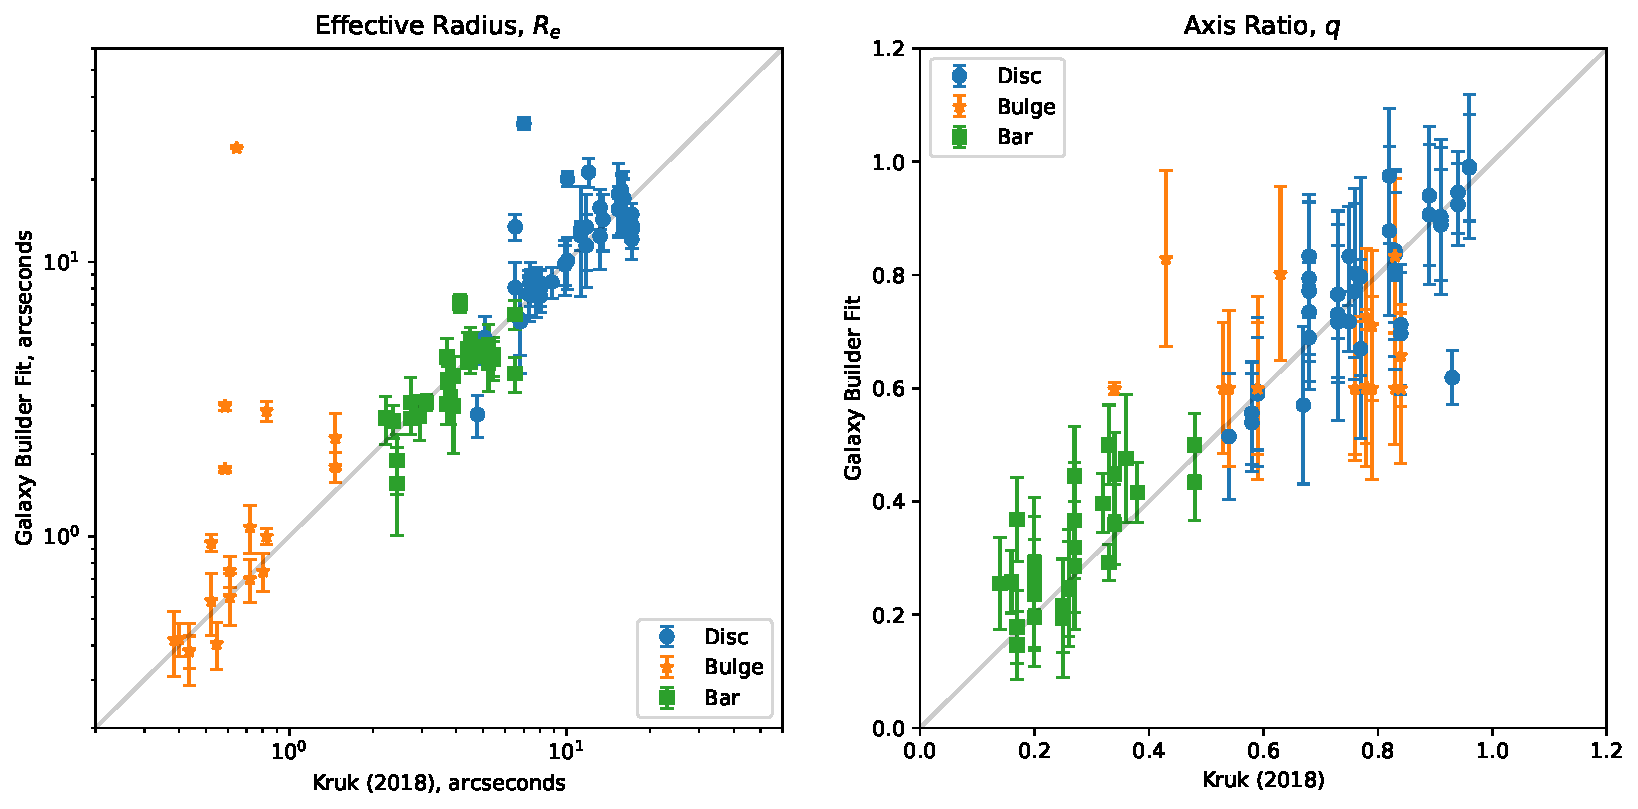
\includegraphics[width=8cm]{images__results/sd_comp_comparison_fitted.pdf}
  \caption{Comparison between \textit{Galaxy Builder} fit models and the result of 3-component, multi\-wavelength fits performed by \citet{2018MNRAS.473.4731K}. Discs, Bulges and Bars are shown as blue circles, orange stars and green squares respectively. The left panel compares component effective radius, the right panel compares the component axis ratio.}
  \label{fig:sd_comp_comparison}
\end{figure}


\subsubsection{Comparison to Disc-Bulge-Bar-Spiral models}
To the best of our knowledge, no photometic models exist for the Galaxy Builder sample which contain spiral arm structure. The closest comparable result is that produced by \citet{Gao2017:1709.00746v1}, however the galaxies they used are not in the Sloan footprint.

In order to provide a comparison for our novel method of spiral parameter (pitch angle and amplitude) extraction, we compare the result of our logarithmic spiral fit to the relationship obtained by \citet{Hart2016:1607.01019v1} between GZ2 classification and galaxy pitch angle (Figure \ref{fig:hart_pitch_angle}). Their fit was obtained by using the Zooniverse to filter good vs bad spiral arm segments identified using a leading automated spiral arm detection and fitting tool, \textsc{SpArcFiRe} \citep{Davis2014:1402.1910v1}, whereas \textit{Galaxy Builder} asks volunteers to provide their own opinion on spiral arm number, location and tightness. \textit{Galaxy Builder} pitch angles are within the uncertainties on the \citet{Hart2016:1607.01019v1} fit, even when not accounting for error on our measurements.

Many researches (\citealt{Davis2014:1402.1910v1}, \citealt{2019arXiv190804246D} to name a few) have noted that many galaxies show large inter-arm variations in pitch angle, suggesting that obtaining a single value of a galaxy's pitch angle is highly dependent on which arms have been identified. We plan to further explore this issue in a future work.

\begin{figure}
  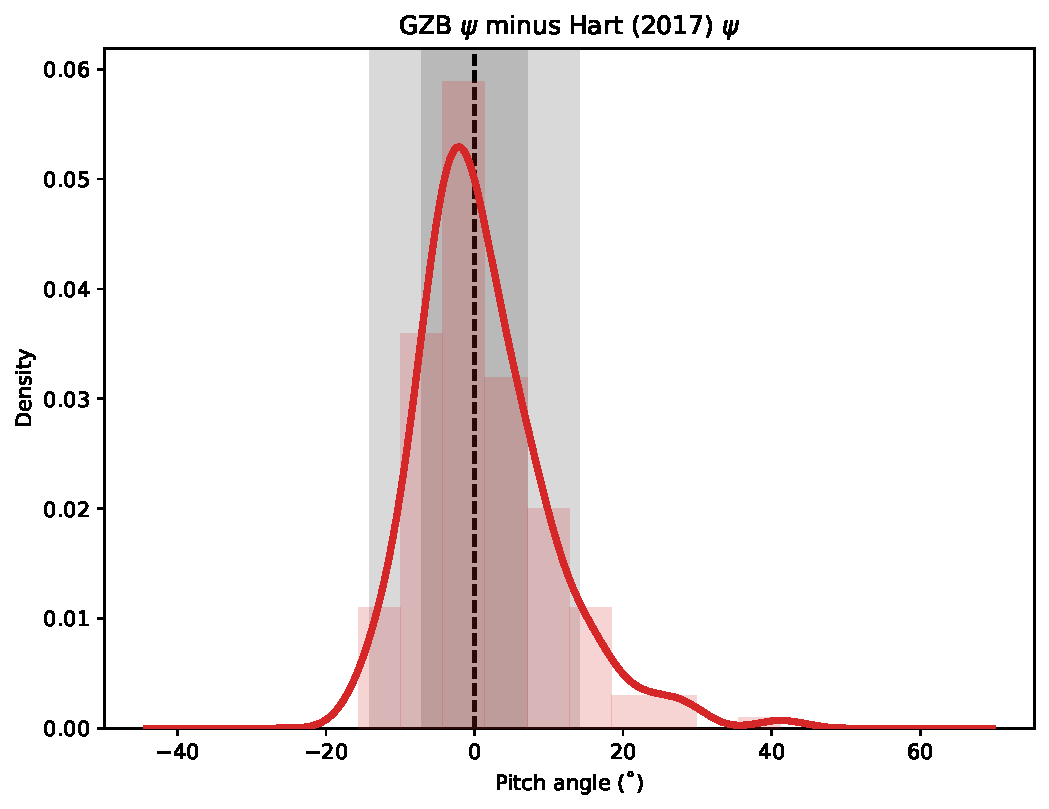
\includegraphics[width=8cm]{images__results/gzb-hart-comparison.pdf}
  \caption{A comparison of Pitch angle obtained by \citet{Hart2016:1607.01019v1} with measured pitch angles for the aggregated model results in galaxies in the Galaxy Zoo Builder sample. The grey regions show 1- and $2\sigma$ errors from \citet{Hart2016:1607.01019v1}. Errors on \textit{Galaxy Builder}-measured pitch angles are not accounted for.}
  \label{fig:hart_pitch_angle}
\end{figure}

\end{document}
